% Generated from the Notion page by tools/notion2tex.py (see report/README.md).
\section{Verification \& Deployment}\label{sec:5}

The preceding design space exploration selected the C22 architecture: Winograd on Conv1, DSP packing on Conv2, 10-bit fixed point and a whole-network dataflow pipeline, with a co-simulated frame time of 1.365 ms at the routed 5 ns clock. This section integrates the exported IP into a PS+PL system on the KV260, verifies it on the board against the contract and gates defined in Section~\ref{sec:3}, and then traces the measured on-board time back to the RTL figure one factor at a time: the PL clock, the software control path, the hardware cycle count, and the external memory path.

\subsection{System integration in Vivado}\label{sec:5.1}

The IP generated by Vitis was imported into a newly created Vivado project, after which we proceeded to create the Block Design. In the Design view, we added the imported srcnn module together with the Zynq UltraScale+ MPSoC, and then ran Block Automation. The PS interface settings used for the SRCNN system are listed in Table~\ref{tab:10}.

\begin{table}[!htbp]
\centering
\footnotesize
\caption{Zynq UltraScale+ PS configuration for the SRCNN block design. Only one master (HPM0) and one slave (HP0) port and a single PL clock are enabled in the first deployment.}
\label{tab:10}
\begin{tabularx}{\linewidth}{llY}
\toprule
PS Configuration & Settings & Purpose \\
\midrule
M\_AXI\_HPM0\_FPD & Enabled & Allows the PS to access SRCNN and the subsequent GPIO control registers \\
S\_AXI\_HP0\_FPD & Enabled, 128bit & The SRCNN master port accesses DDR through the PS \\
M\_AXI\_HPM1\_FPD & Disabled & Not used \\
PL0 & Enabled, 200 MHz requested & Provides the clock for SRCNN and the AXI interconnect \\
PL1 & Disabled & Not used in baseline \\
\bottomrule
\end{tabularx}
\end{table}

After configuring the PS interfaces, we connected the control path and the data path separately. The PS's \texttt{M\_AXI\_HPM0\_FPD} accesses the \texttt{s\_axi\_control} interface of SRCNN through a control SmartConnect; SRCNN's \texttt{m\_axi\_image\_in}, \texttt{m\_axi\_parameters}, and \texttt{m\_axi\_image\_out} are connected to \texttt{S\_AXI\_HP0\_FPD} through another SmartConnect to access the PS's DDR.

The resulting block design is shown in Figure~\ref{fig:7}.

\begin{figure}[!htbp]
\centering
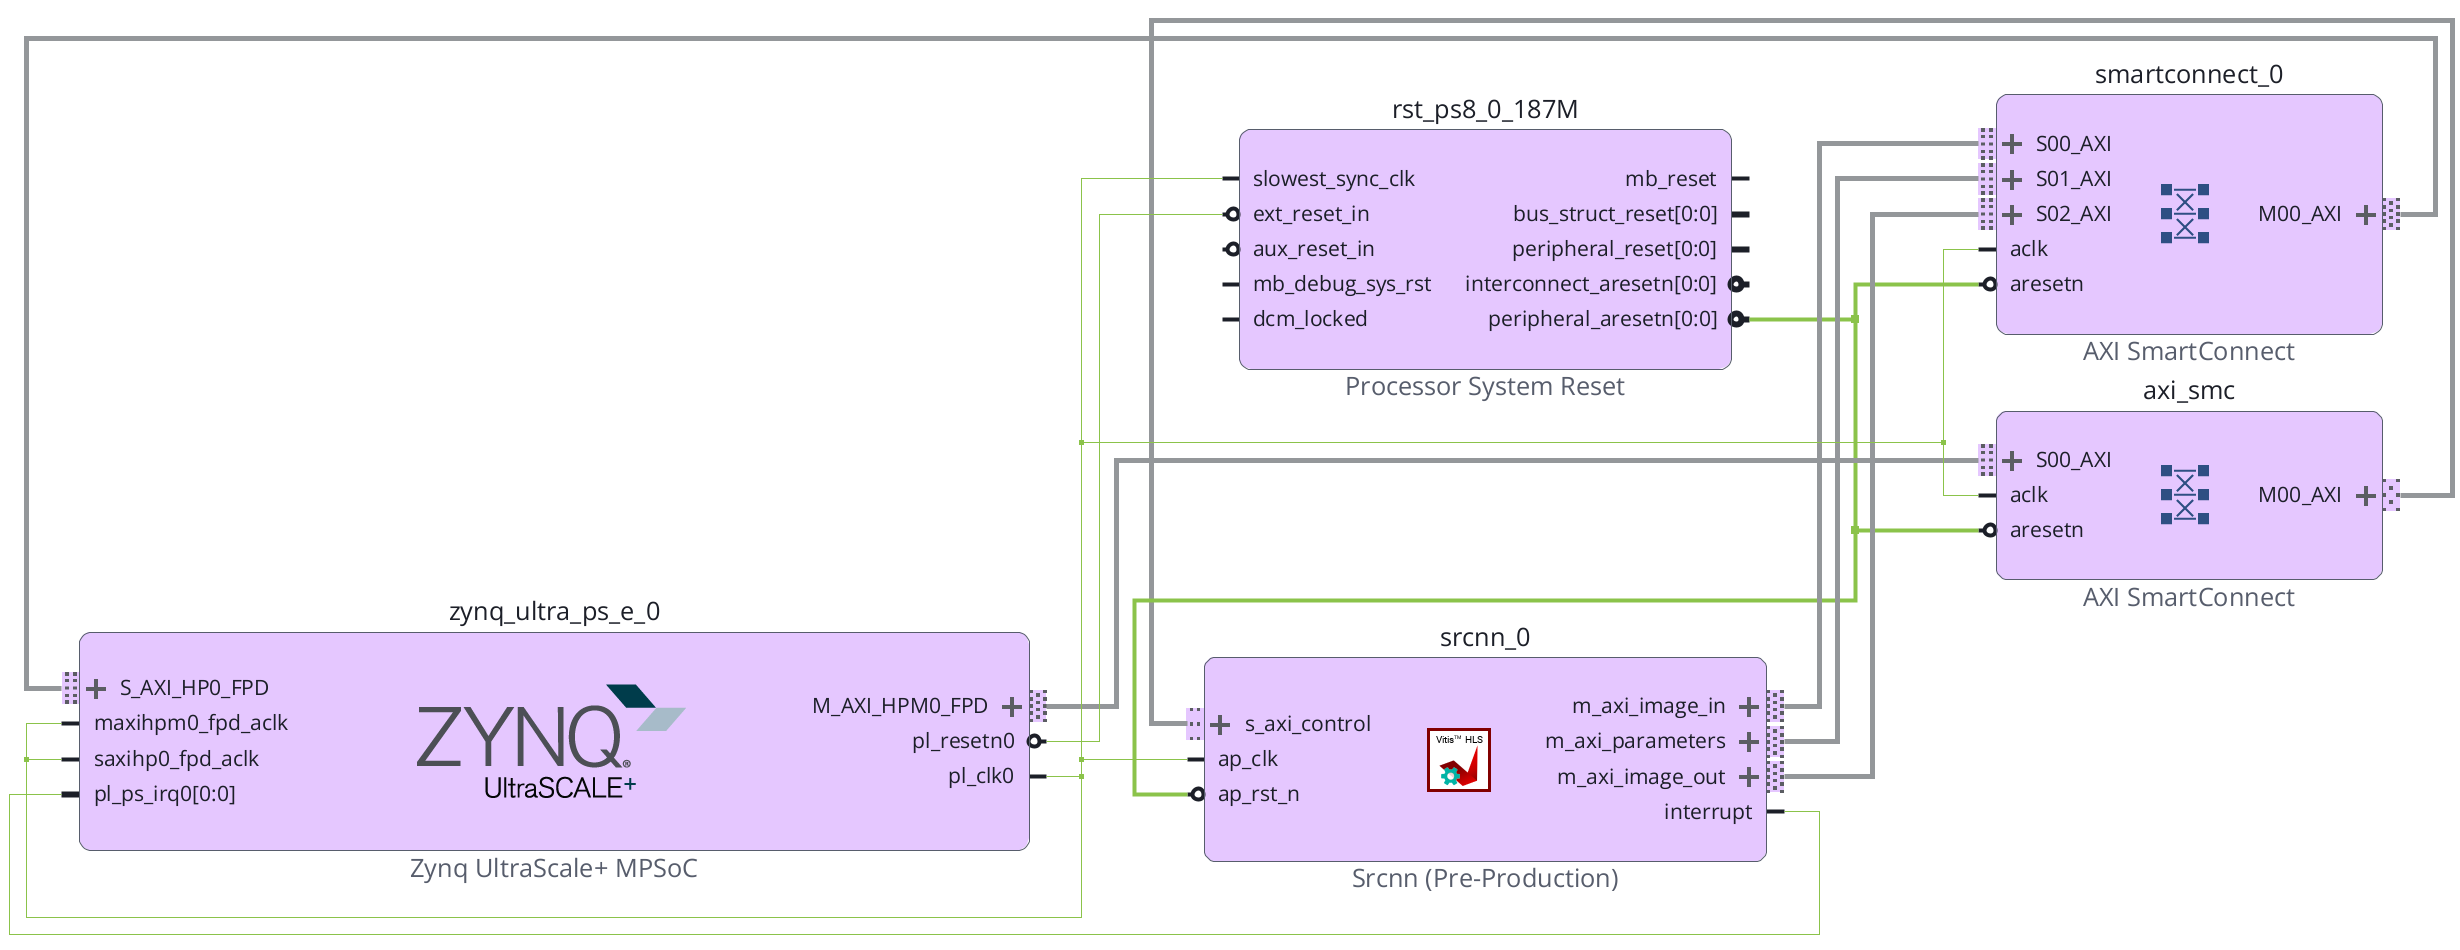
\includegraphics[width=\figw]{figures/fig07-block-design-hp0.png}
\caption{Vivado block design of the first PS+PL deployment. The PS reaches the SRCNN control registers through M\_AXI\_HPM0\_FPD and a control SmartConnect; the three SRCNN AXI masters (image\_in, parameters, image\_out) share S\_AXI\_HP0\_FPD through a second SmartConnect.}
\label{fig:7}
\end{figure}

The post-route resource utilization of this design is given in Table~\ref{tab:11}.

\begin{table}[!htbp]
\centering
\footnotesize
\caption{Post-route resource utilization of the C22 design on the xck26-sfvc784-2LV-c device, as reported by Vivado after implementation.}
\label{tab:11}
\begin{tabular}{lrrr}
\toprule
Resource & Usage & Available & Utilization (\%) \\
\midrule
LUT & 63,078 & 117,120 & 53.86\% \\
FF & 106,341 & 234,240 & 45.40\% \\
DSP & 1,032 & 1,248 & 82.69\% \\
BRAM36 & 54.5 & 144 & 37.85\% \\
Used CLB & 14,309 & 14,640 & 97.74\% \\
\bottomrule
\end{tabular}
\end{table}

Vivado implements the integrated system at the PL0 period it derives from the PS preset, 5.333 ns (187.5 MHz). At this constraint the post-route report shows WNS +0.043 ns, WHS +0.010 ns, TNS = THS = 0, no unconstrained endpoints, all 181,382 nets routed and zero routing errors, so the final gate of Section~\ref{sec:3} is satisfied by the integrated system as well as by the stand-alone IP (C22: WNS +0.013 ns at 5 ns). The worst setup path lies in the Conv1 Winograd engine (4.893 ns data path, of which 3.127 ns logic and 1.766 ns routing), and the slack of 43 ps shows the timing margin leaved by the T = 4 is quite small. Vivado's power model estimates 5.8 W on chip (5.5 W dynamic, of which 2.6 W is the PS). The resource utilization in Table~\ref{tab:11} shows why no further growth of the design is possible: the DSPs are 82.7 \% used and the CLBs 97.7 \%, so the device is effectively full.

\subsection{Functional verification on the board}\label{sec:5.2}

The bitstream and the hardware handoff file were loaded on the KV260 through PYNQ 3.0.1. One invocation proceeds as follows: contiguous buffers are allocated for the input image, the six parameter arrays and the output; the float32 weights and biases are copied in the exact layout of the HLS function signature; the output buffer is filled with NaN; all buffers are flushed to DDR; the buffer addresses are written to the IP's control registers; the IP is started and \texttt{AP\_DONE} is polled; the output buffer is invalidated and read back; and the result is compared against the reference. Two timers wrap this sequence: \emph{start-to-done} covers only the interval between the start write and the observation of \texttt{AP\_DONE}, and \emph{with cache and copy} covers the whole invocation including cache maintenance, the copy of the output and the NaN/Inf check.

We compared the output content of the FPGA board in two ways: first, a bit-by-bit comparison with the results computed by co-simulation to verify whether the hardware computation results are correct. Image quality is then measured against the float golden output and the ground-truth image as MSE and PSNR; this tells us what the fixed-point design costs in quality. Table~\ref{tab:12} traces each specification and gate from Section~\ref{sec:3} to the on-board evidence that closes it.

\begin{table}[!htbp]
\centering
\footnotesize
\caption{Specifications and acceptance gates from Section~\ref{sec:3}}
\label{tab:12}
\begin{tabularx}{\linewidth}{L{4.6cm}L{3.1cm}Y}
\toprule
Specification / gate (Section~\ref{sec:3}) & Expected & Measured on the board \\
\midrule
\texttt{srcnn} signature with float arrays, runtime-loaded parameters & Parameters read from DDR on every call & Constant-image test with altered weights and biases returns the analytically expected value 104/256; restoring the original parameters restores the bit-exact output \\
Bit-exact against the fixed-point reference on all 13 Set14 images & 13 / 13 & 13 / 13, plus Butterfly (Set5) \\
Mean PSNR on Set14 no worse than $-$0.1 dB against float & $\ge$ $-$0.1 dB & 29.083 dB on the board, identical to the C17 co-simulation record (29.083 dB); $-$0.076 dB against the float golden (Section~\ref{sec:4}) \\
Post-route timing met, zero unrouted nets & Met at the implemented clock & Met at 5.333 ns: WNS +0.043 ns, WHS +0.010 ns, 0 route errors; +0.074 ns with the cycle monitor added \\
Primary metric: milliseconds per frame & 1.365 ms at 200 MHz (RTL $\times$ routed clock) & 2.938 ms hardware time at 166.665 MHz \\
\bottomrule
\end{tabularx}
\end{table}

Table~\ref{tab:13} lists the per-image result of the Set14 run. The mean PSNR against the ground truth matches the co-simulation record to three decimals. The per-image start-to-done time is essentially constant at 2.95 ms, as expected.

\begin{table}[!htbp]
\centering
\footnotesize
\caption{Set14 verification on the KV260 (output on HP1, 166.665 MHz). Bit-exact is against the fixed-point reference output of each image; PSNR is against the ground-truth image, for the bicubic input and for the SRCNN output; gain is the difference. Time is the Python start-to-done interval of the single run.}
\label{tab:13}
\begin{tabular}{llrrrr}
\toprule
Image & Bit-exact & PSNR input (dB) & PSNR output (dB) & Gain (dB) & Start-to-done (ms) \\
\midrule
baboon & True & 27.36 & 27.89 & +0.53 & 2.953 \\
barbara & True & 24.90 & 24.97 & +0.07 & 2.951 \\
bridge & True & 25.23 & 26.18 & +0.95 & 2.954 \\
coastguard & True & 26.30 & 26.82 & +0.52 & 2.950 \\
face & True & 32.68 & 33.34 & +0.66 & 2.952 \\
flowers & True & 25.70 & 27.30 & +1.60 & 2.952 \\
foreman & True & 33.20 & 35.48 & +2.28 & 2.950 \\
lenna & True & 29.17 & 30.78 & +1.61 & 2.950 \\
man & True & 26.06 & 27.09 & +1.03 & 2.952 \\
monarch & True & 24.58 & 27.97 & +3.39 & 2.952 \\
pepper & True & 32.05 & 33.35 & +1.31 & 2.950 \\
ppt3 & True & 26.68 & 29.34 & +2.66 & 2.951 \\
zebra & True & 24.74 & 27.56 & +2.82 & 2.952 \\
\textbf{Mean} & \textbf{13 / 13} & \textbf{27.59} & \textbf{29.08} & \textbf{+1.49} & \textbf{2.951} \\
\bottomrule
\end{tabular}
\end{table}

The \textbf{parameter reload test} zeroes all weights, sets the biases to 0.5, 0.25 and 0.125, places a single 0.25, 0.5 and 0.5 at the centre of one kernel in each layer, and feeds a constant 0.5 image; the expected output is then a constant (0.5 $\times$ 0.25 + 0.5) $\times$ 0.5 + 0.25 = 0.5625 $\rightarrow$ $\times$ 0.5 + 0.125 = 104/256 after quantization, and the board returns exactly this value, which shows that the parameters are read from DDR on every call rather than cached from the first. Restoring the original parameters restores the bit-exact Butterfly output. The \textbf{NaN pre-fill} of the output buffer ensures that an IP that never writes a pixel is detected, since the check fails on any remaining NaN.

\subsection{Performance debugging}\label{sec:5.3}

Functionally the design was therefore correct from the first bitstream, but the inference time of the initial deployment was 5.05 ms per image, 3.7$\times$ the 1.365 ms of the RTL reference. Three causes were suspected: the operating clock, the Python control and polling overhead, and the AXI/DDR access path. The following subsections take them in order.

\subsubsection{Clock frequency}\label{sec:5.3.1}

First, we read the clock frequency: on the board, PYNQ was used to read \texttt{Clocks.fclk0\_mhz}, which returned \texttt{124.99875 MHz}. This is reasonable. Although PL0's requested frequency was set to \texttt{200 MHz} in Vivado, the actual configured frequency recorded in the HWH is \texttt{187.498123 MHz}, with the clock source being the IOPLL and a divider ratio of \texttt{8$\times$1}. \texttt{IOPLL\_CTRL = 0x13c00} corresponds to a multiplier of 60 with the output divided by 2. Therefore, based on a reference clock of approximately \texttt{33.333 MHz}, the on-board IOPLL runs at about \texttt{1000 MHz}, and the PL0 frequency is about \texttt{1000 $\div$ 8 = 125 MHz}. In contrast, the Vivado preset uses an IOPLL of about 1500 MHz, so the same divider yields about \texttt{187.5 MHz}. At the 125 MHz actually configured, the 273,023 RTL cycles would take 2.18 ms, so the clock alone explains less than half of the 5.05 ms.

We changed the divider to 6 and observed that the time was further reduced to 3.98 ms; Table~\ref{tab:14} compares the two clock configurations.

\begin{table}[!htbp]
\centering
\footnotesize
\caption{PL0 clock configuration before and after changing the IOPLL output divider from 8 to 6. The frequency is derived from the PLL control registers read on the board; the time is the median Python start-to-completion time over repeated runs.}
\label{tab:14}
\begin{tabular}{lll}
\toprule
Parameter & Before Modification & After Modification \\
\midrule
PL0 divider & 8$\times$1 & 6$\times$1 \\
Register-derived frequency & 124.99875 MHz & 166.665 MHz \\
Median time from start to completion & 5.005195 ms & 3.984220 ms \\
Output consistent with reference & True & True \\
\bottomrule
\end{tabular}
\end{table}

We deliberately stopped at a divider of 6 rather than going to 5 (200 MHz). The purpose of this step was to measure how strongly the on-board time depends on the PL clock, not to reach the design clock; the PL0 clock also drives the AXI interconnect, so a change cannot be attributed to the compute logic alone, and a run at 200 MHz would first need its own timing verification on the integrated system. To separate clock-bound from clock-independent time, we swept the divider over 10, 8 and 6 in alternating order (four sweeps, five timed runs each after a warm-up) with the three AXI masters still sharing HP0; Table~\ref{tab:15} gives the result.

\begin{table}[!htbp]
\centering
\footnotesize
\caption{PL0 clock sweep with the three AXI masters sharing HP0. Median, minimum and maximum of 20 start-to-done measurements per frequency; software-equivalent cycles = median time $\times$ frequency; RTL reference = 273,023 cycles $\div$ frequency.}
\label{tab:15}
\begin{tabular}{lrrrR{2.3cm}R{1.9cm}}
\toprule
PL0 clock (MHz) & Median (ms) & Min (ms) & Max (ms) & Software-equivalent cycles & RTL reference (ms) \\
\midrule
99.999 & 5.955 & 5.950 & 5.957 & 595,460 & 2.730 \\
124.999 & 4.994 & 4.992 & 4.997 & 624,290 & 2.184 \\
166.665 & 3.982 & 3.977 & 3.984 & 663,688 & 1.638 \\
\bottomrule
\end{tabular}
\end{table}

From the output, we found: The time falls with frequency, but not in proportion: the software-equivalent cycle count rises from 595 k to 664 k as the clock rises, so a part of the time does not scale with the PL clock. A linear fit \emph{t = a + b / f} to the three points gives \emph{b} $\approx$ 493 k cycles and \emph{a} $\approx$ 1.0 ms: roughly 493 k cycles of the work run on the PL clock, and about 1 ms per frame is spent in a path whose latency is fixed in absolute time, which points at the PS-side interconnect and the DDR controller rather than at the accelerator. This indicates that AXI/DDR overhead is what dominates the hardware execution time, the hardware counters below confirm it.

\subsubsection{Software overhead: register access and polling}\label{sec:5.3.2}

We then looked at the time spent on Python reads/writes and polling. A single read via \texttt{ip.read(0x00)} took 7.807 \textmu{}s, compared with 2.353 \textmu{}s via \texttt{ip.mmio.array[0]}; both are negligible against a frame time of several milliseconds. To test whether the polling itself disturbs the execution (for example through MMIO traffic on the same interconnect), we delayed the first status read by 0, 1, 2 and 3 ms after the start write, ten repeats each, and recorded the completion time and the number of status reads (Table~\ref{tab:16}).

\begin{table}[!htbp]
\centering
\footnotesize
\caption{Effect of delaying the first status read after the start write (HP0 configuration, 166.665 MHz; medians of 10 runs). The completion time is unchanged while the number of polling reads falls from 606 to 135, so polling does not affect the execution.}
\label{tab:16}
\begin{tabular}{lrrr}
\toprule
Requested first wait (ms) & Actual first read (ms) & Median completion (ms) & Median polling reads \\
\midrule
0 & 0.013 & 3.981 & 606.5 \\
1 & 1.106 & 3.984 & 443.0 \\
2 & 2.100 & 3.984 & 288.5 \\
3 & 3.100 & 3.983 & 135.0 \\
\bottomrule
\end{tabular}
\end{table}

The completion time is identical to within 3 \textmu{}s regardless of the polling density, so neither register access nor polling contributes to the gap. Software overhead is therefore confined to the part of the invocation outside the start-to-done interval, which is reported separately in Table~\ref{tab:20}.

\subsubsection{Hardware cycle count}\label{sec:5.3.3}

Neither the clock frequency nor the software path can account for the gap between on-board and simulated execution times, and the clock sweep suggested a clock-independent component. It passively observes the write channel of the SRCNN \texttt{s\_axi\_control} slave (AWADDR, AWVALID/AWREADY, WDATA, WSTRB, WVALID/WREADY) and the SRCNN \texttt{interrupt} output. The counter starts on the clock edge at which a write to \texttt{AP\_CTRL} with bit 0 set is accepted, counts PL0 cycles, and stops and latches on the edge at which the completion interrupt is observed. The 32-bit count and a status word (completion sequence number, busy, overflow and error flags) are brought out through a dual-channel AXI GPIO on the control SmartConnect, which the PS reads after each run; the sequence number lets the software confirm that the count belongs to the frame just launched. The interval includes a few cycles of control and interrupt latency on either side of the true \texttt{ap\_start} $\rightarrow$ \texttt{ap\_done} window, which is negligible against the hundreds of thousands of cycles in question. The new build was re-checked: WNS +0.074 ns, THS = TPWS = 0. The block design with the cycle monitor is shown in Figure~\ref{fig:8}.

\begin{figure}[!htbp]
\centering
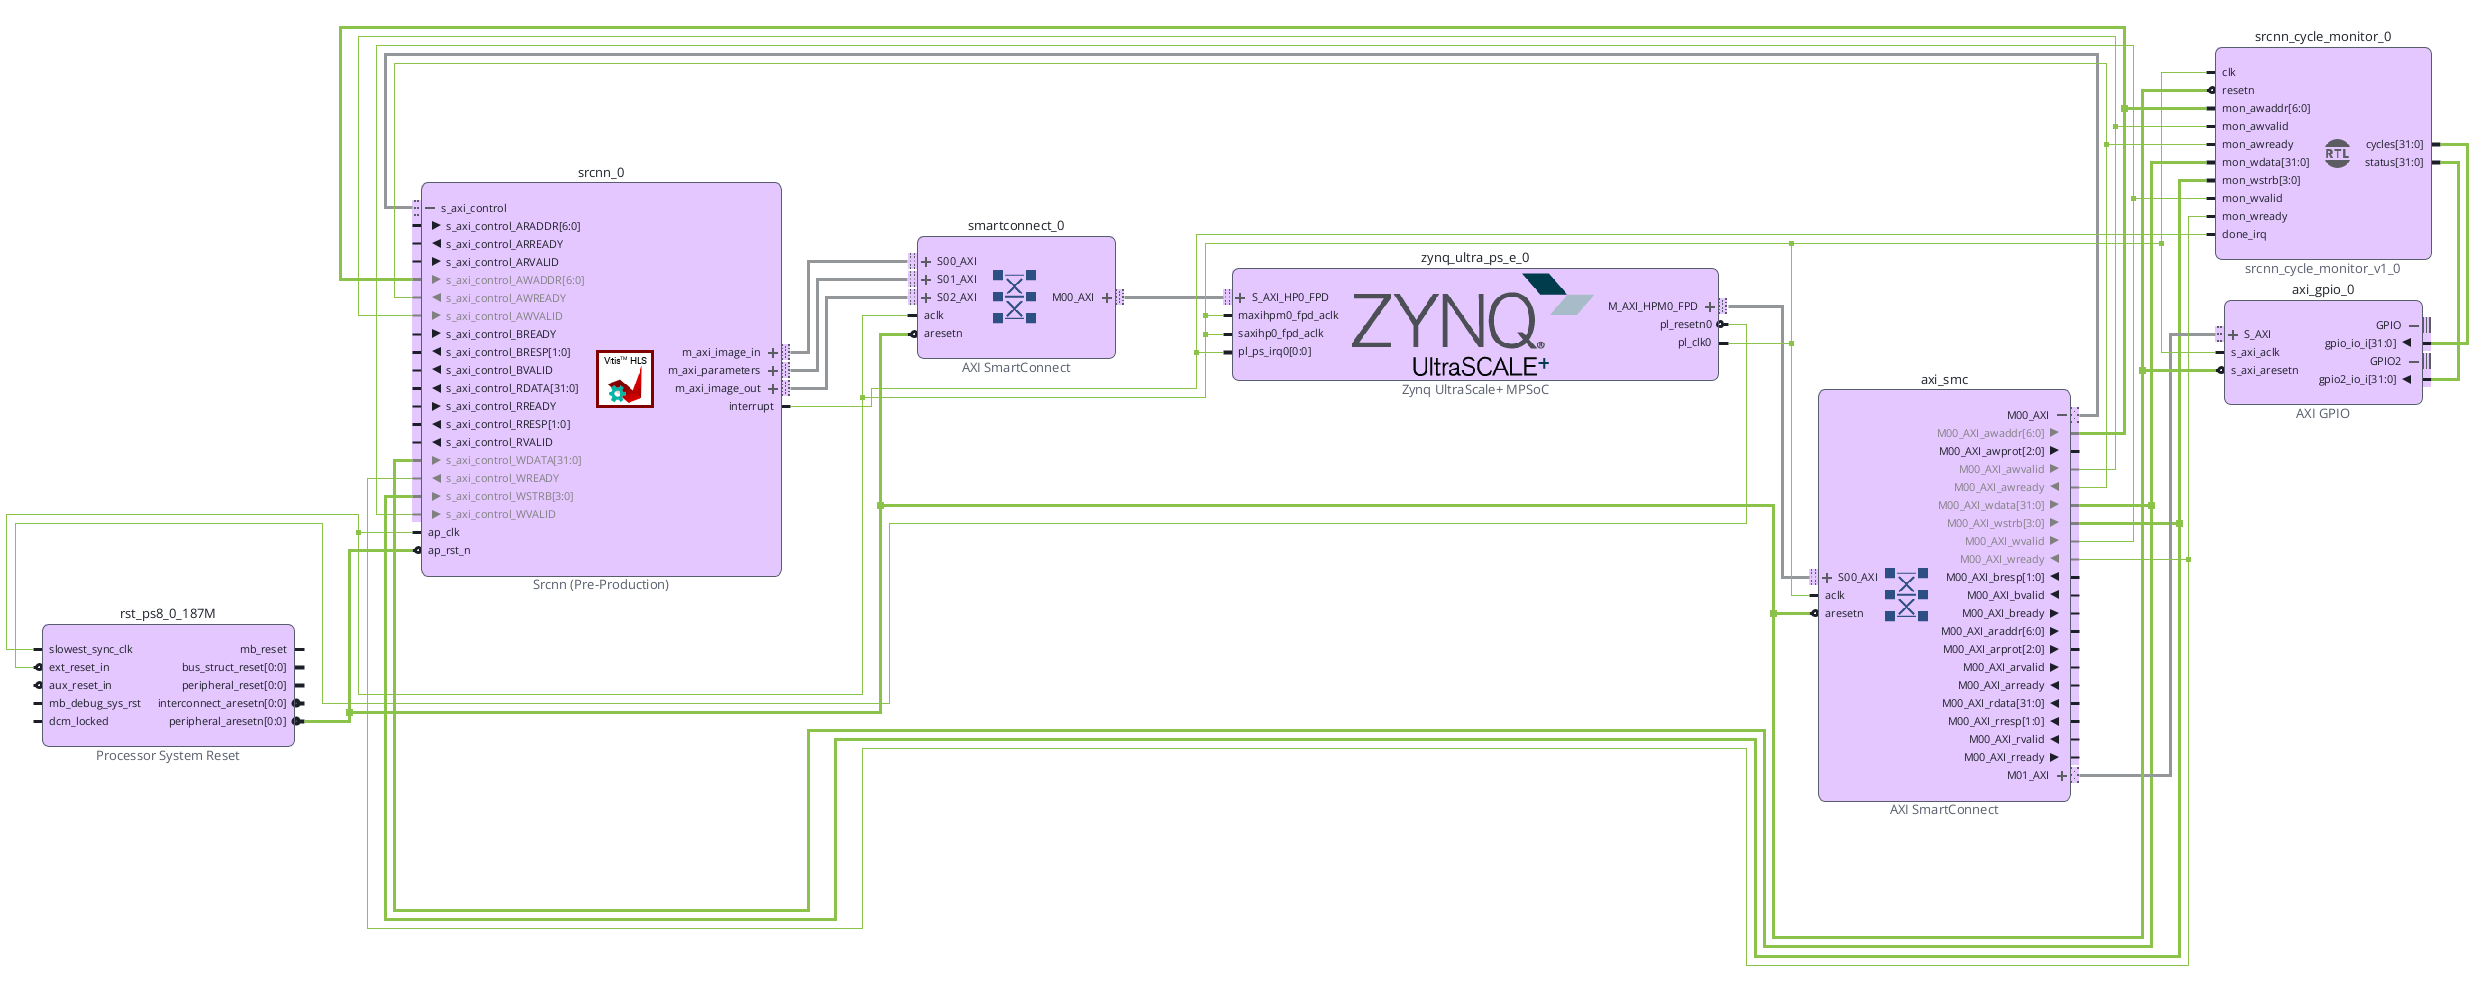
\includegraphics[width=\figw]{figures/fig08-block-design-cycle-monitor.png}
\caption{Block design with the hardware cycle-monitor module. The counter starts on the start write to the SRCNN s\_axi\_control interface and stops and latches on the SRCNN completion interrupt, so the count excludes all PYNQ software overhead.}
\label{fig:8}
\end{figure}

The measurement it produced is summarized in Table~\ref{tab:17}.

\begin{table}[!htbp]
\centering
\footnotesize
\caption{Hardware-timed execution of one frame measured by the cycle monitor at 166.665 MHz, compared with the Python-timed start-to-completion interval.}
\label{tab:17}
\begin{tabular}{ll}
\toprule
Metric & Result \\
\midrule
Operating frequency & 166.665 MHz \\
Hardware count & 668,366 cycles \\
Hardware-timed interval & 4.010236 ms \\
Python start-to-completion time & 4.033060 ms \\
Difference between the two & 22.824 \textmu{}s \\
Output bit-exact with reference & True \\
\bottomrule
\end{tabular}
\end{table}

The original RTL reference is 273,023 cycles, while 668,366 cycles were measured on the board --- an excess of 395,343 cycles. RTL co-simulation results show that the Dataflow pipeline of the three SRCNN convolution layers already achieves high computational unit utilization, and the RTL execution cycles are close to the HLS estimate. Therefore, the time gap relative to simulation is caused at the hardware execution level. Considering that on-board operation also involves the AXI interconnect, HP ports, and DDR controller, we further examine the external memory access path to determine whether there is additional data transfer waiting.

\subsubsection{Memory access path}\label{sec:5.3.4}

To check whether the shared AXI access path introduces additional wait time, we tried splitting the output path: the image output was connected to the 128-bit \texttt{S\_AXI\_HP1\_FPD} through an independent SmartConnect, while the input and parameters still access HP0 through the original SmartConnect. The modified block design is shown in Figure~\ref{fig:9}.

\begin{figure}[!htbp]
\centering
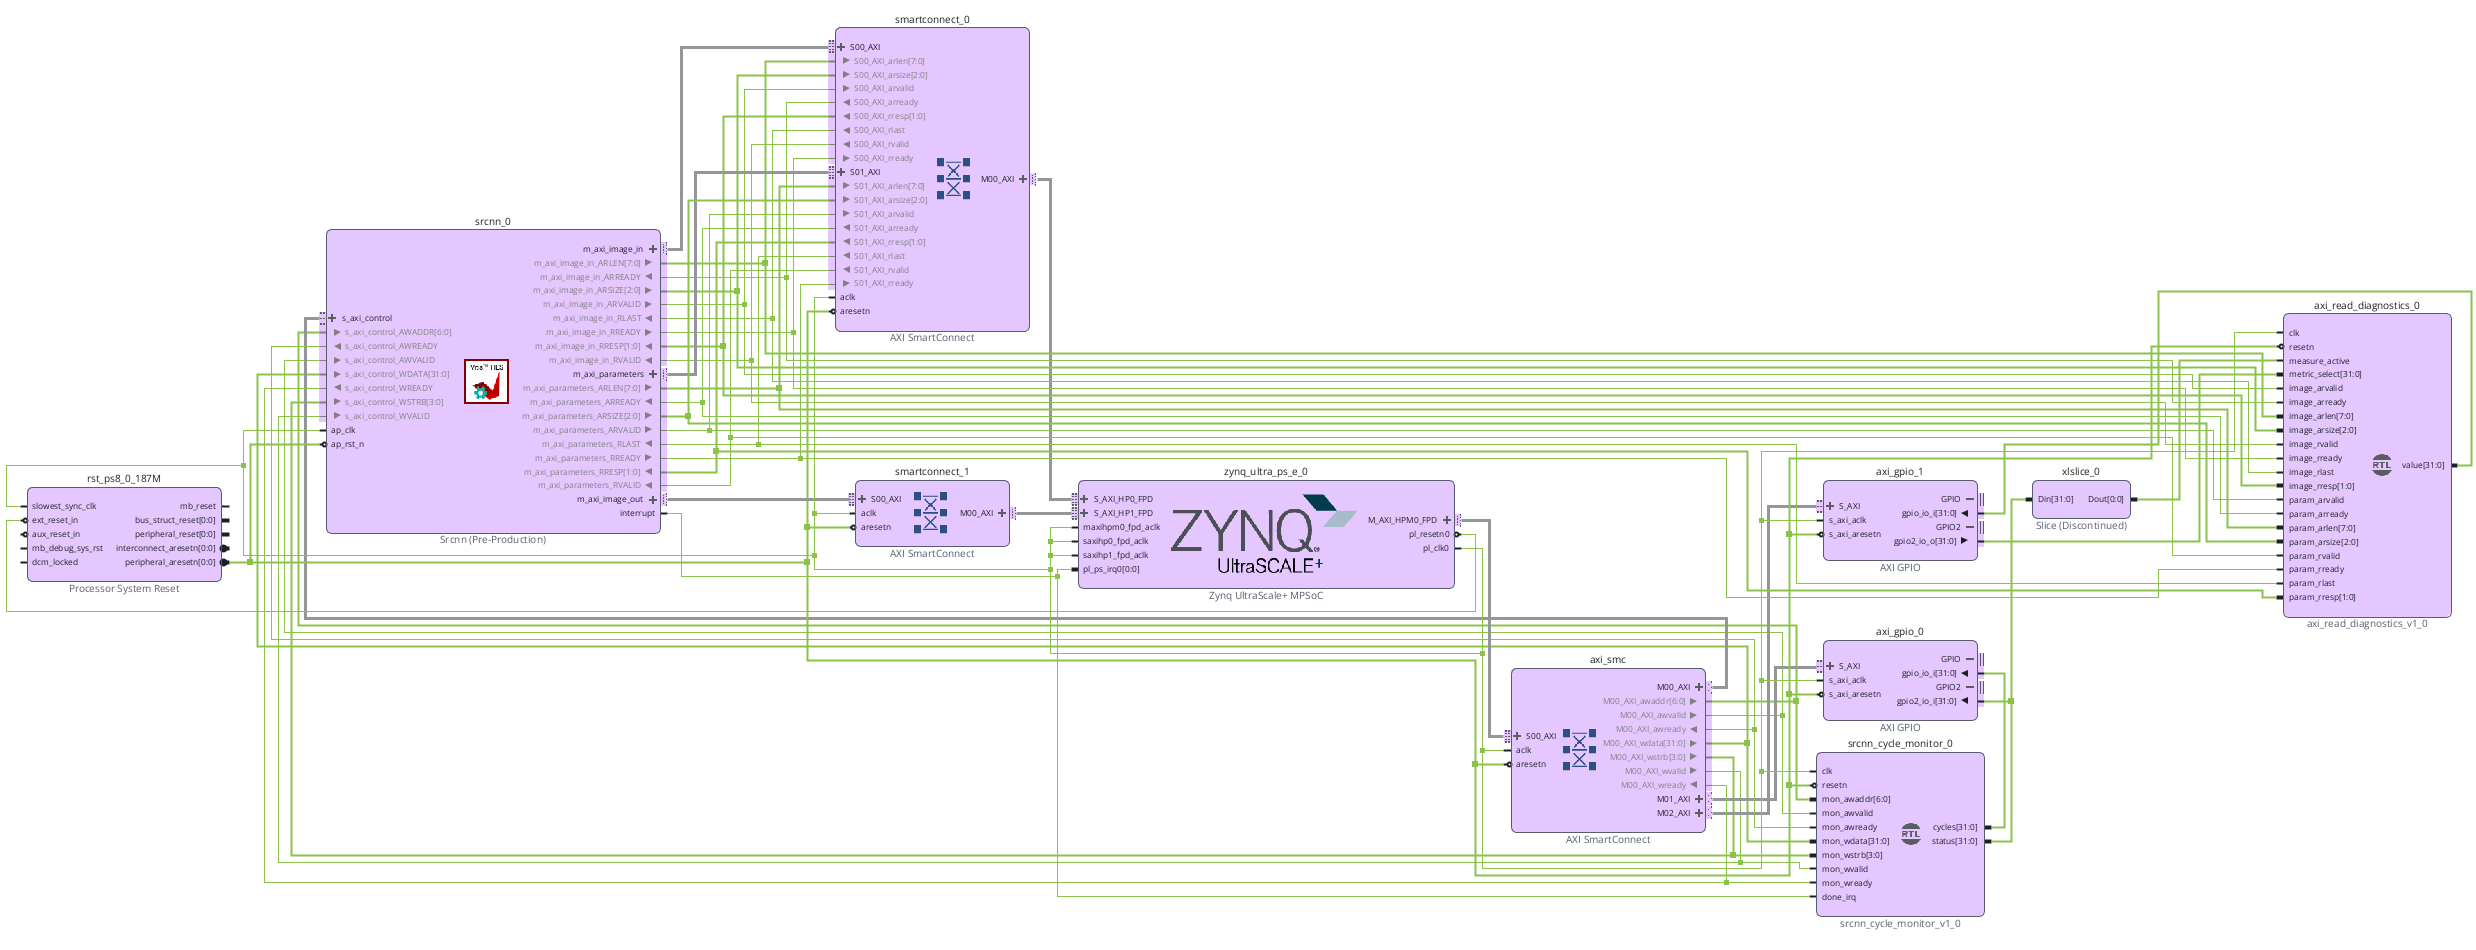
\includegraphics[width=\figw]{figures/fig09-block-design-hp1.png}
\caption{Block design with the output path separated: m\_axi\_image\_out reaches DDR through its own SmartConnect and S\_AXI\_HP1\_FPD, while m\_axi\_image\_in and m\_axi\_parameters keep sharing S\_AXI\_HP0\_FPD. The cycle monitor from Figure~\ref{fig:8} is retained.}
\label{fig:9}
\end{figure}

The design still passed verification at 166.665 MHz, and the on-board execution time dropped to 2.94 ms, with the cycle count reduced to 489,585. Table~\ref{tab:18} compares the two configurations over repeated runs; separating the output path reduces the hardware cycle count by 26.6 \%.

\begin{table}[!htbp]
\centering
\footnotesize
\caption{On-board cycle count and hardware time per frame with the three AXI masters sharing HP0 (Figure~\ref{fig:8}) versus the output on a dedicated HP1 port (Figure~\ref{fig:9}). Minimum, median and maximum are taken over repeated runs at 166.665 MHz.}
\label{tab:18}
\begin{tabular}{lll}
\toprule
Metric & Three interfaces sharing HP0 & Output on dedicated HP1 \\
\midrule
Minimum cycles & 666,988 & 489,423 \\
Median cycles & 667,084 & 489,584.5 \\
Maximum cycles & 668,015 & 497,301 \\
hardware time & 4.003 ms & 2.938 ms \\
Output bit-exact & True & True \\
\bottomrule
\end{tabular}
\end{table}

This is one of the main reasons why the actual execution time exceeds the simulated time. AMD's official documentation also notes that the Zynq UltraScale+'s HP interfaces reach the DDR controller through an interconnect network, and that accesses are subject to arbitration and QoS mechanisms.\footnote{AMD Xilinx wiki, \emph{Traffic Shaping of HP Ports on Zynq UltraScale+}: \url{https://xilinx-wiki.atlassian.net/wiki/spaces/A/pages/688128001/Traffic\%2BShaping\%2Bof\%2BHP\%2BPorts\%2Bon\%2BZynq\%2BUltraScale}}

To further pinpoint the problem, we added an AXI read-path statistics module. For each of the image and parameter ports it observes ARVALID/ARREADY, ARLEN, ARSIZE, RVALID/RREADY, RLAST and RRESP, and accumulates sixteen counters over the busy window of the cycle monitor: window cycles, accepted read requests, returned data beats, completed bursts, requested beats and bytes, cycles of AR back-pressure (ARVALID without ARREADY), cycles of R back-pressure (RVALID without RREADY, the HLS consumer not accepting data), cycles with a request outstanding but no RVALID, the maximum number of outstanding transactions, first-AR and last-RLAST cycle, non-OKAY responses, orphan RLASTs and outstanding transactions at the end of the window. The counters are selected and read through a second AXI GPIO after the frame completes; the read-back script checks the frame sequence number, that requested beats equal returned beats, and that no response errors or outstanding transactions remain before the numbers are used. The average burst length is returned beats divided by completed bursts. The block design with this module added is shown in Figure~\ref{fig:10}.

\begin{figure}[!htbp]
\centering
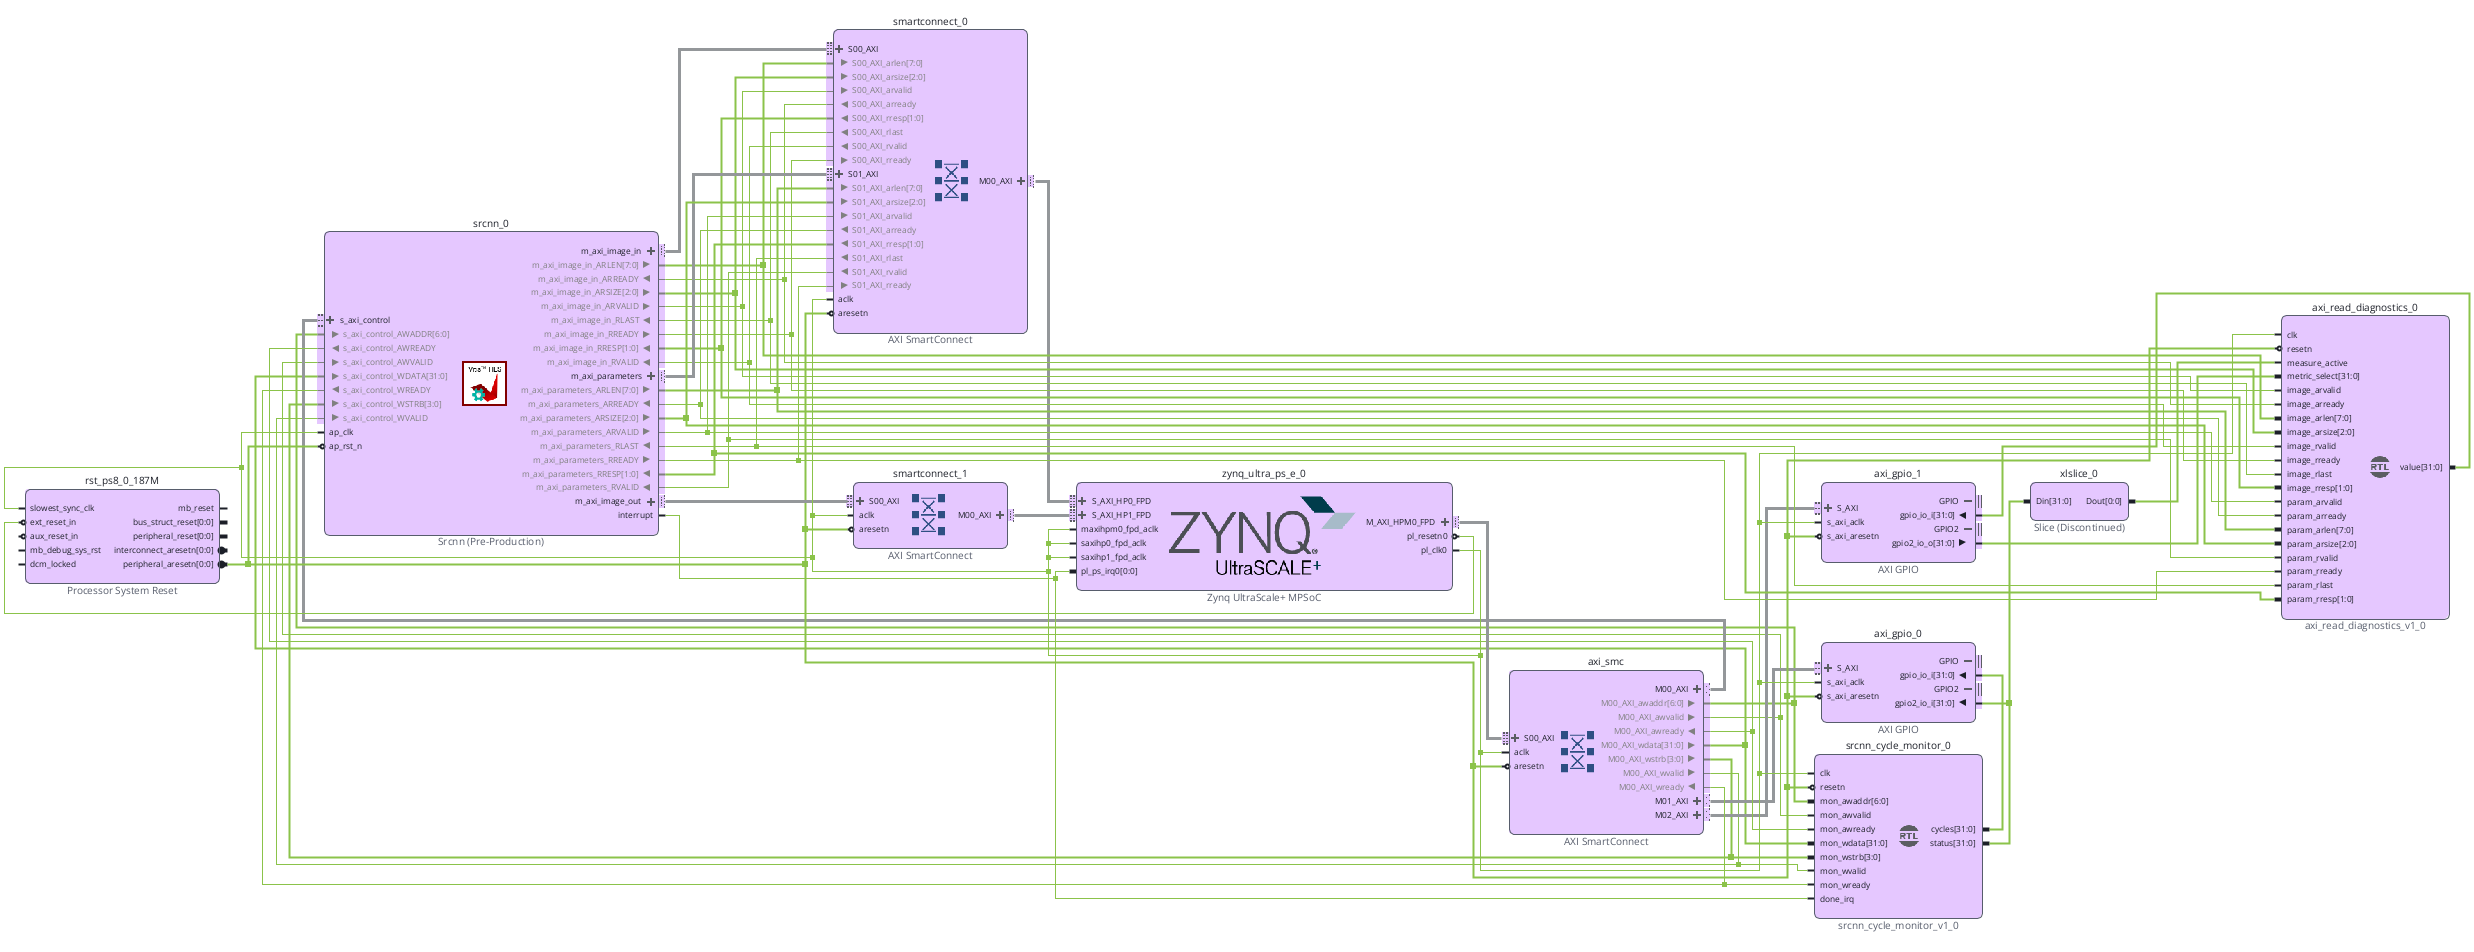
\includegraphics[width=\figw]{figures/fig10-block-design-axi-stats.png}
\caption{Block design with the AXI read-path statistics module attached to the image and parameter read channels on HP0. The module counts total cycles, cycles with an outstanding read request but no valid data, and the average burst length of each channel; the output path remains on HP1 as in Figure~\ref{fig:9}.}
\label{fig:10}
\end{figure}

With this module in place, the run on the FPGA board executed a total of 494,066 cycles, taking about 2.964 ms. Among these, the image input channel had outstanding read requests without valid data returned during approximately 77.7\% of the statistics window cycles, indicating that there are substantial read-response gaps during image reading. In addition, the average burst length of both read channels was 1 beat, showing that the actual AXI reads did not form multi-beat bursts. Although we set \texttt{max\_read\_burst\_length=256} in HLS, this parameter only specifies the maximum allowed burst length; the actual bursts are not controlled by this parameter.

The section of the AMD official documentation mentioned earlier, which discusses the impact of AXI access patterns on the transfer performance of the Zynq UltraScale+ HP interfaces, also supports our hypothesis: the currently observed read-response gaps may be related to the transfer overhead caused by single-beat transactions, as well as the access latency in the AXI interconnect, the HP interfaces, and the DDR controller.

\subsection{Final on-board result}\label{sec:5.4}

\begin{table}[!htbp]
\centering
\footnotesize
\caption{Per-frame latency of the SRCNN accelerator at each stage of development and deployment. The RTL reference is co-simulated cycles $\times$ 5 ns; all other rows are measured on the KV260.}
\label{tab:19}
\begin{tabularx}{\linewidth}{llY}
\toprule
Stage & Latency & Description \\
\midrule
Original floating-point Baseline & 2.238 s & Measured on board \\
Final architecture RTL reference & 1.365 ms & Simulation cycles $\times$ 5 ns \\
First on-board deployment & 5.05 ms & Initial clock configuration \\
After clock adjustment & 3.984 ms & 166.665 MHz \\
After input/output splitting & 2.938 ms & Final on-board hardware time \\
\bottomrule
\end{tabularx}
\end{table}

Table~\ref{tab:19} summarizes the execution latency of the SRCNN accelerator across different development and deployment stages. The original floating-point baseline requires 2.238 s to run one frame on the board. After optimizations such as fixed-point quantization, Winograd convolution, and the Dataflow pipeline, the final architecture achieves an estimated execution time of 1.365 ms in RTL simulation. However, the actual latency of the first on-board deployment is 5.05 ms, significantly higher than the simulation result.

By adjusting the PL clock frequency and separating the output data path from the shared HP0 interface to an independent HP1 interface, the on-board execution latency is reduced to 2.938 ms, a 762$\times$ speedup over the original baseline measured on the same board. Table~\ref{tab:20} characterises this final configuration over 20 consecutive runs, and Figure~\ref{fig:11} shows its reconstructed image.

\begin{table}[!htbp]
\centering
\footnotesize
\caption{Timing of the final configuration (output on HP1, PL0 at 166.665 MHz) over 20 consecutive Butterfly runs, all bit-exact. Start-to-done is the Python-timed interval from the start write to the observation of AP\_DONE; with cache and copy is the complete invocation. The hardware-timed value from the cycle monitor (Table~\ref{tab:18}) is 2.938 ms.}
\label{tab:20}
\begin{tabular}{llrl}
\toprule
Quantity & Min & Median & Max \\
\midrule
Start-to-done (ms) & 2.949 & 2.951 & 2.958 \\
With cache and copy (ms) & 5.907 & 5.976 & 6.549 \\
Hardware cycles (cycle monitor) & 489,423 & 489,584.5 & 497,301 \\
RTL reference at 166.665 MHz (ms) & --- & 1.638 & --- \\
\bottomrule
\end{tabular}
\end{table}

The Python start-to-done median of 2.951 ms exceeds the hardware-timed 2.938 ms by 13 \textmu{}s, which is the cost of the start write and the last status read; the two timers agree, so the software timer can be used as a proxy for hardware time in the earlier experiments where the cycle monitor was not yet present.

\begin{figure}[!htbp]
\centering
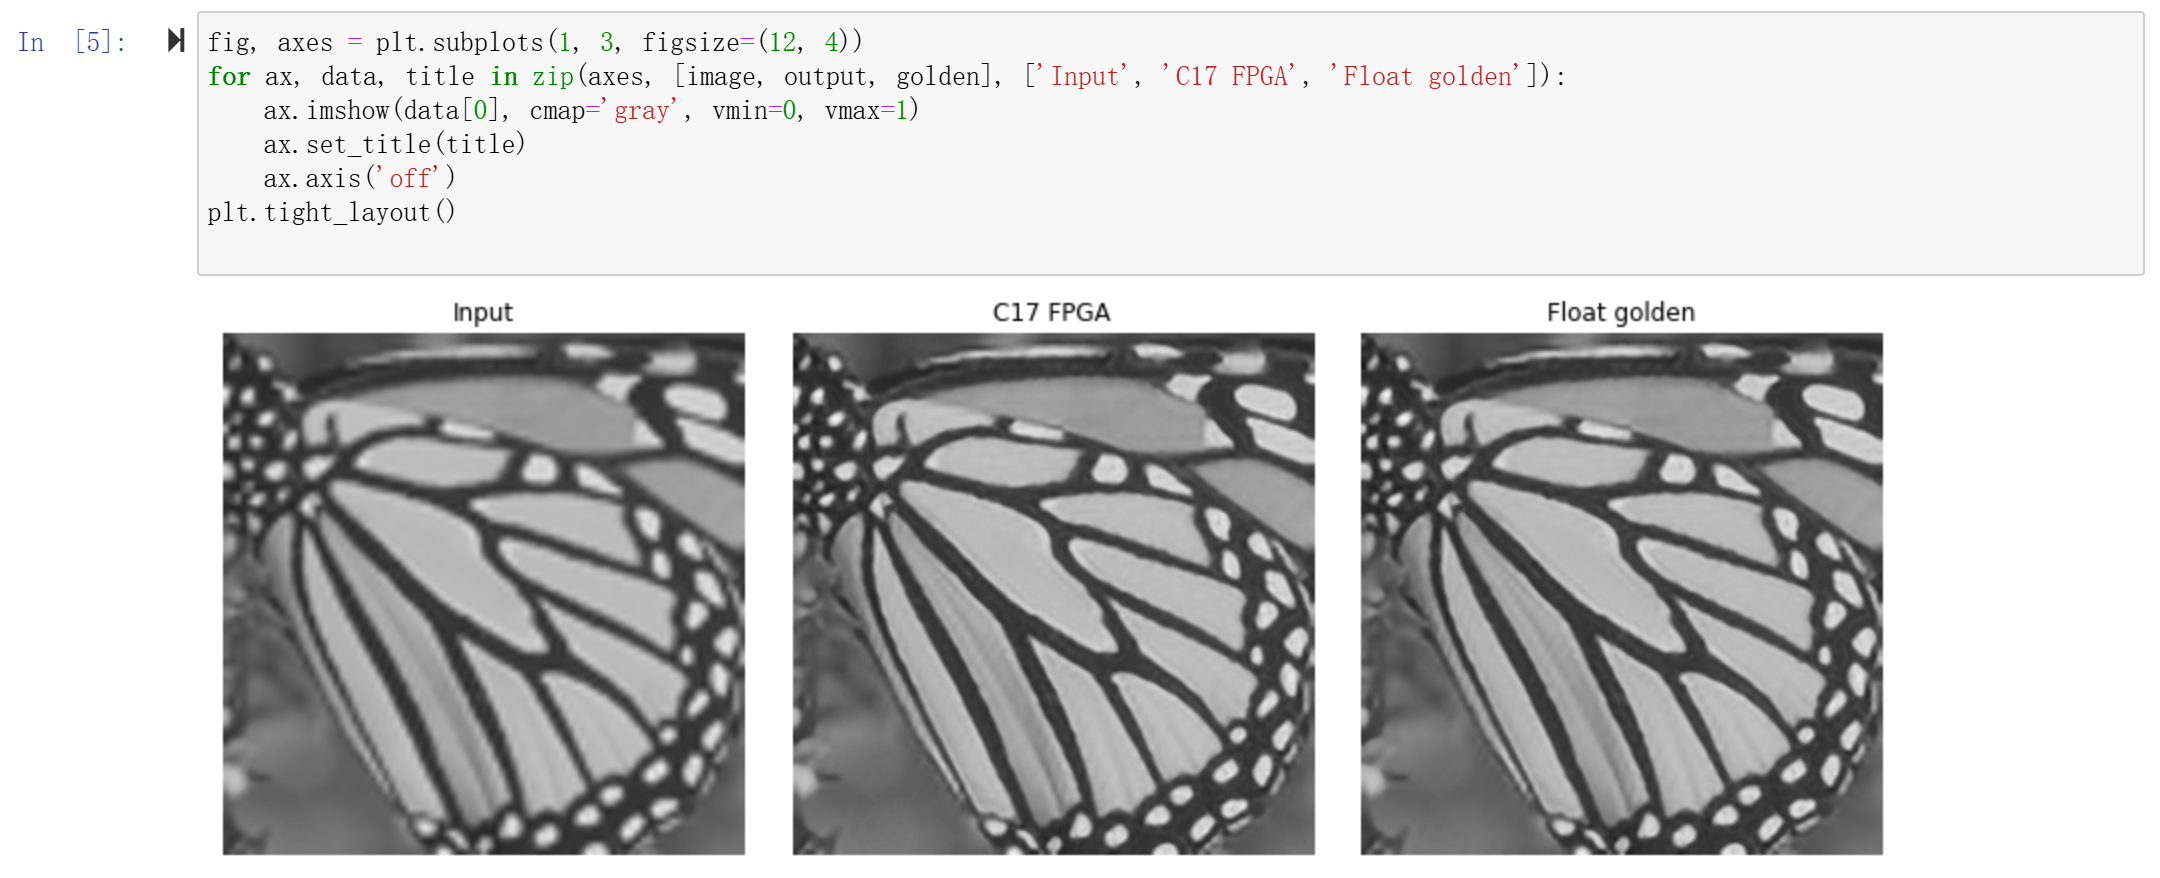
\includegraphics[width=\figw]{figures/fig11-butterfly.png}
\caption{Butterfly: bicubic input (left), output of the final version running on the KV260 (centre, output on HP1, 166.665 MHz) and float golden (right). The board output is bit-exact with the fixed-point reference; MSE against the float golden is 1.77 $\times$ 10\textsuperscript{-5}.}
\label{fig:11}
\end{figure}

Figure~\ref{fig:11} shows the Butterfly input, the board output and the float golden side by side; the board output is bit-exact with the fixed-point reference and its MSE against the float golden is \texttt{1.77065 $\times$ 10\textsuperscript{-5}}. The median hardware execution time is \texttt{2.938 ms} (489,584.5 cycles, about 340 frames per second). A complete invocation takes about 6 ms (median 5.98 ms, Table~\ref{tab:20}); the 3 ms beyond the hardware time is spent in the software control flow: filling the output buffer with NaN, flushing the input and parameter buffers to DDR, writing the address registers, invalidating and re-reading the output after completion, copying it out and checking for NaN or Inf. The two numbers answer different questions and should be kept apart: the hardware time is the performance of the accelerator, the invocation time is the performance of the present PYNQ driver around it, and only the former is the primary metric of Section~\ref{sec:3}.
